\section{Signalflussdiagramme (SFD)}{53}

\textbf{Grafische Darstellungen von linearen Gleichungssystemen}


\subsection{Definitionen}{53-54}

\begin{center}
    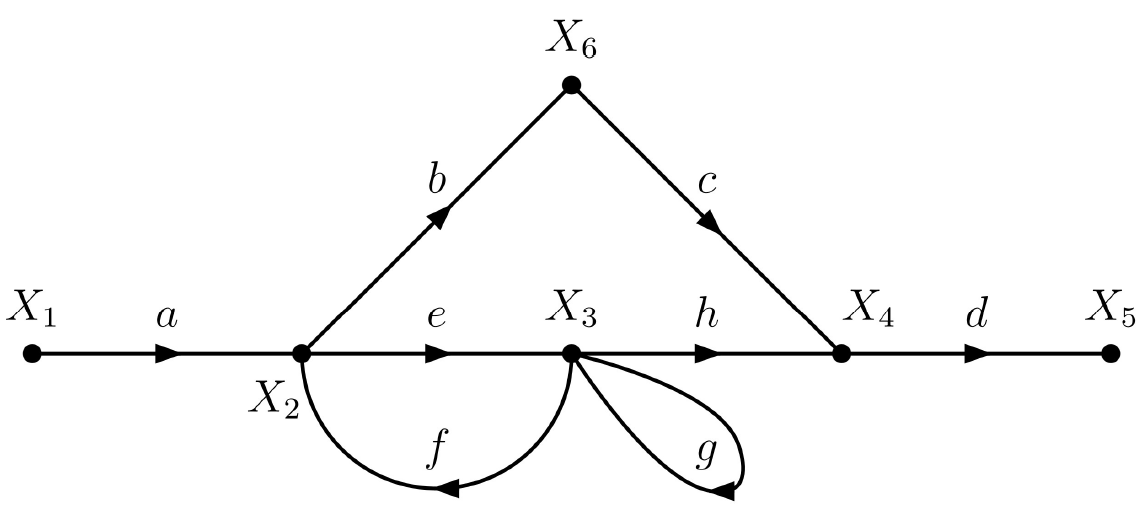
\includegraphics[width=0.75\columnwidth]{images/signalflussdiagramm.png}
\end{center}


\cbl{Der Wert einer Variablen, (Knoten) berechnet sich durch \textbf{Addition} der Zweige, die in diesen Knoten \textbf{einmünden}} 
$$\cbl{ X_4 = h \cdot X_3 + c \cdot X_6 } $$

\vspace{0.2cm}

\begin{itemize}
    \setlength\itemsep{5pt}

    \item \textbf{Knoten} Stellt bestimmte Grösse (Variable) dar ($X_1, \, X_2, \, ...$)
    \item \textbf{Zweig} Gerichete Stecke stellt funktionale Abhängigkeit zwischen Knoten dar
    \item \textbf{Quelle} Knoten ohne einmündende Zweige ($X_1$) stellen unabh. Variable dar
    \item \textbf{Senke} Knoten ohne weggehende Zweige ($X_5$) stellen Variable dar, von welcher keine andere Variable im System abhängt
    \item \textbf{Gemischter Knoten} Knoten mit hineinführenden und weggehenden Zweigen ($X_2, \, X_3, \, X_4, \, X_6$)
    \item \textbf{Pfad} Kontinuierliche Folge von Zweigen, welche alle in die gleiche Richtung zeigen ($abcd, \, aef, \, bcd \, \ldots$)
    \item \textbf{Offener Pfad} Pfad, bei dem jeder beteiligte Knoten nur \textbf{einmal} durchquert wird
    \item \textbf{Vorwärtspfad} Offener Pfad zw. Quelle und Senke oder einem gemischten Knoten
    \item \textbf{Schleife} Geschlossener Pfad, welcher zum Ausgangsknoten zurückkehrt ($ef, \, g$)
    \item \textbf{Eigenschleife} Rückkopplungsschleife aus einem Zweig und einem Knoten ($g$)
    \item \textbf{Zweigtransmittanz} Proportianalitätskonstante zwischen zwei Knoten (Vorfaktor von Variable)
    \item \textbf{Schleifentransmittanz} Produkt der Zweigtransmittanzen einer Schleife ($ef, \, g$)
\end{itemize}


\subsection{Konstruktionsregeln}{55}

\begin{itemize}
    \item Variablen stehen bei den Knoten
    \item Signale durchqueren Zweige \textbf{nur} in Pfeilrichtung
    \item \textbf{Multiplikation} mit Transmittanzen
    \item Variable ist \textbf{Summe} der \textbf{einmündenden} Signale
    \item Variable wird auf weitergehende Zweige kopiert
\end{itemize}


\subsection{Reduktionsregeln}{59-71}

Gleichungssysteme können mit den folgenden Regeln vereinfacht werden. Die Vereinfachung entspricht einer \textbf{sukzessiven
Elimination abhängiger Variablen}.


\subsubsection{Kettentransformation}{59}

\begin{center}
    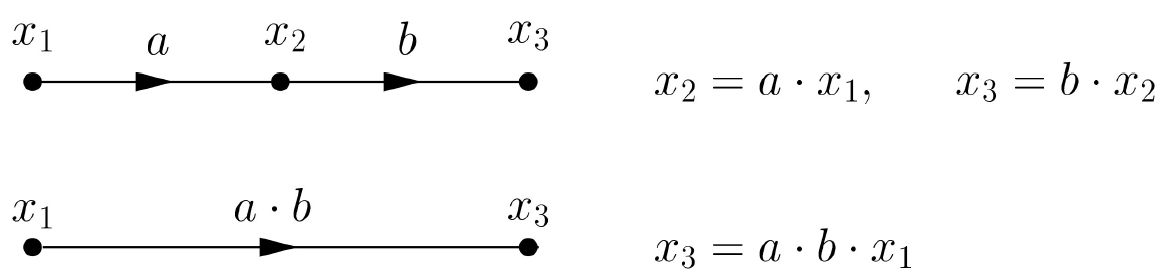
\includegraphics[width=0.8\columnwidth]{images/kettentransformation.png}
\end{center}


\subsubsection{Paralleltransformation}{59}

\begin{center}
    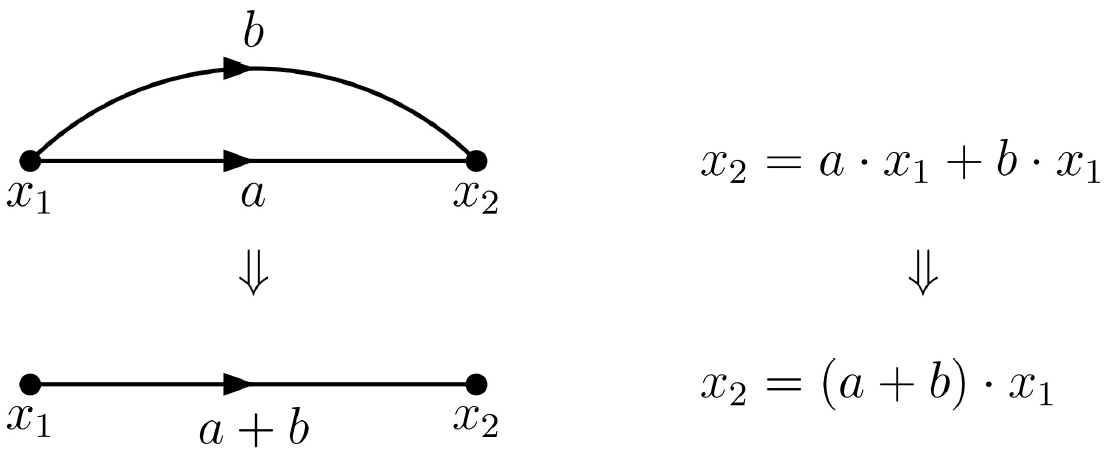
\includegraphics[width=0.7\columnwidth]{images/paralleltransformation.png}
\end{center}


\subsubsection{Entfernung eines Knotens}{60}

\begin{center}
    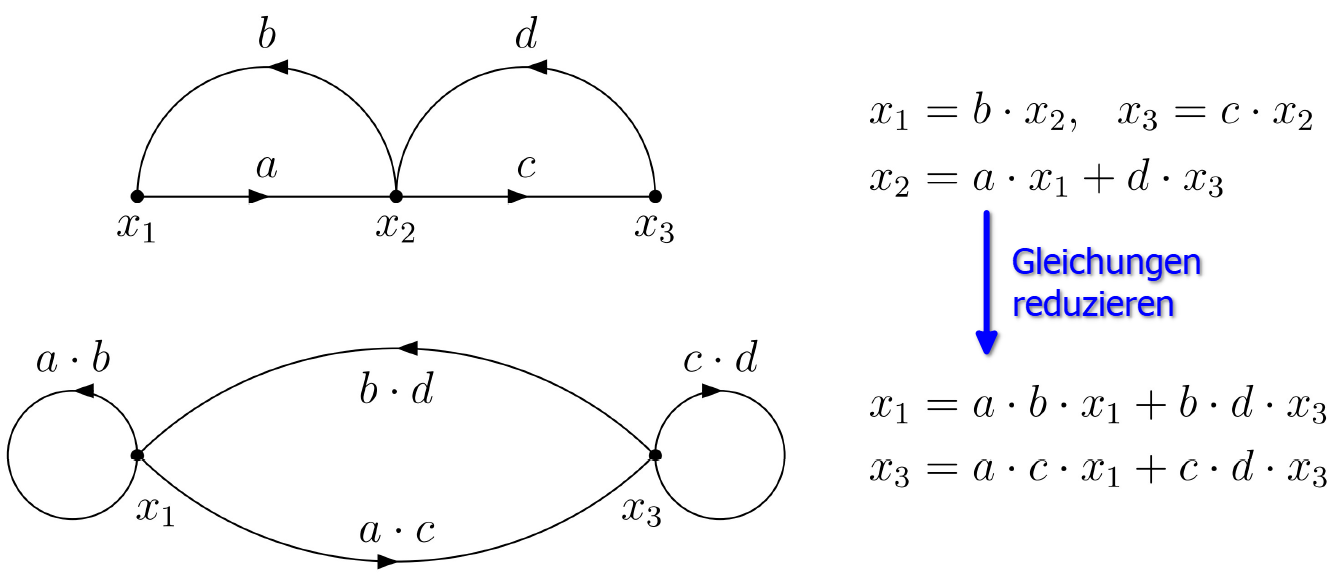
\includegraphics[width=0.85\columnwidth]{images/entfernung_knoten.png}
\end{center}


\subsubsection{Transmittanzverschiebungen}{60-61}

\textbf{Achtung:} Es muss eine neue Variable $\tilde{x_3}$ eingeführt werden, wenn der \textbf{Endpunkt eines inneren Zweiges} 
verschoben wird 

\begin{center}
    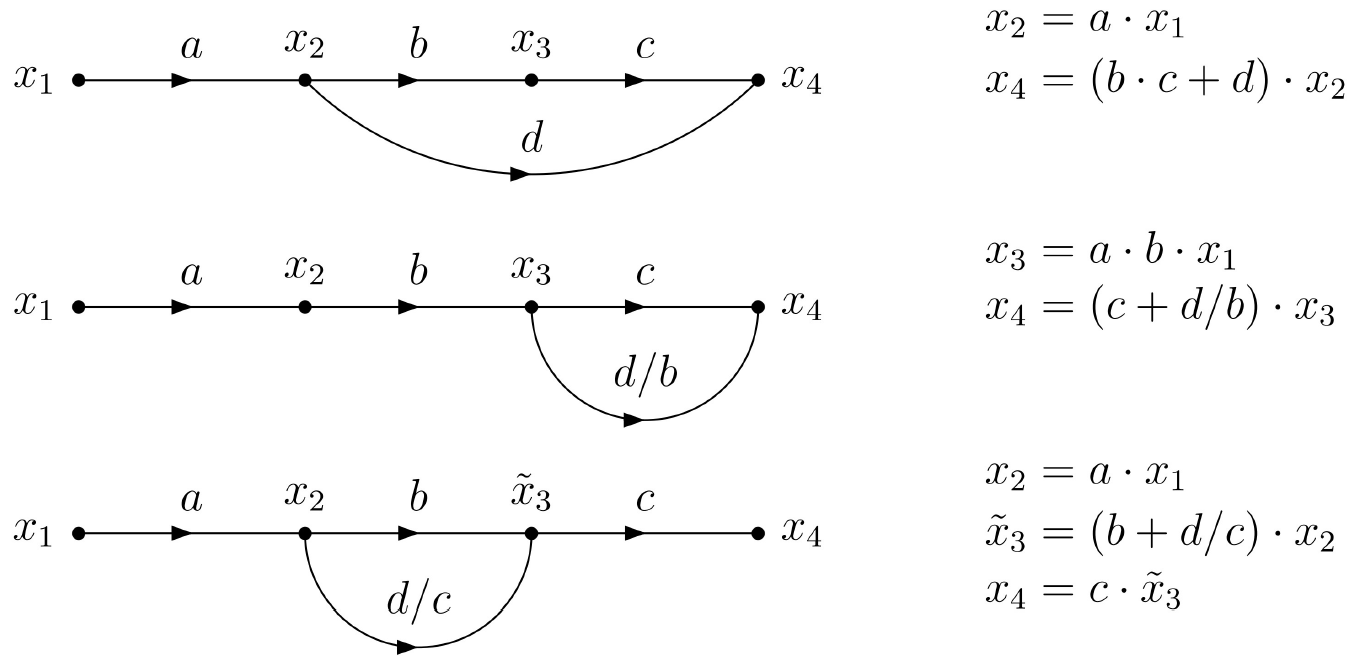
\includegraphics[width=0.85\columnwidth]{images/transmittanzverschiebung_1.png}

    \vspace{0.2cm}

    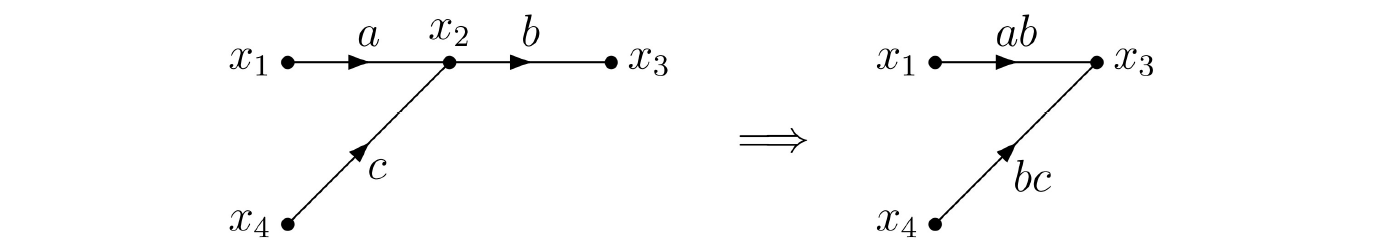
\includegraphics[width=0.75\columnwidth]{images/transmittanzverschiebung_2.png}
\end{center}



\subsubsection{Pfadinversion}{61-62}

Pfad mit Ursprung bei einer \cbl{\textbf{Quelle} $x_i$}, Endpunkt beim \cgn{Knoten $x_j$} und \textcolor{magenta}{Transmittanz $\mu$} \\
invertieren: 

\vspace{0.1cm}

\begin{itemize}
    \item Ersetzung mit Pfad von $x_j$ nach $x_i$ mit Transmittanz $1/\mu$
    \item Alle anderen Zweige, welche ursprünglich bei $x_j$ endeten so verschieben dass sie bei $x_i$ enden und ihre Transmittanzen mit $-1/\mu$ multiplizieren 
\end{itemize}

\begin{center}
    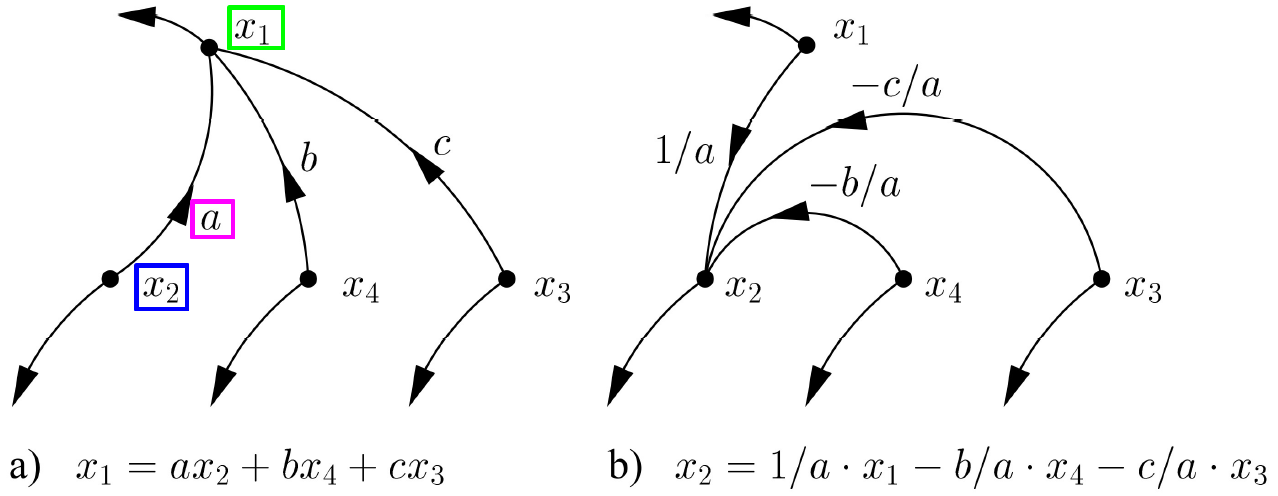
\includegraphics[width=0.9\columnwidth]{images/pfadinversion_2.png}
\end{center}

\textbf{Achtung:} Inversion eines Pfades hat Effekt, dass Quelle vom einen Ende des Pfades zum anderen Ende verschoben wird.\\
\textrightarrow\ Folge von sukzessiven Inversionen



\subsubsection{Entfernung einer Eigenschleife}{62}

Transmittanzen von allen anderen Zweigen, welche in betroffenen Knoten \textbf{einmünden} durch $(1-b)$ dividieren 

\begin{center}
    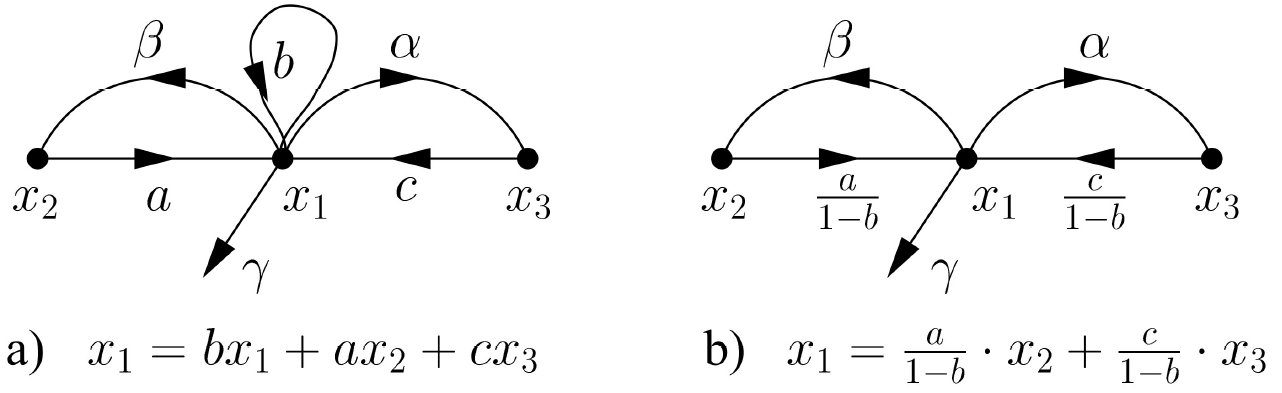
\includegraphics[width=0.8\columnwidth]{images/entfernung_eigenschleife.png} 
\end{center}


\subsubsection{Schleifenreduktion}{63-64}

\myul{\textbf{Einzelne Schleife}}

\vspace{0.1cm}

Die Transmittanz einer unabhängigen Variablen (Quelle) $x_i$ zu einer abhängigen Variablen (innerer Knoten / Senke) in einem SFD,
das nur eine Schleife und einen Vorwärtspfad enthält ist:

\vspace{0.2cm}


\begin{minipage}[c]{0.24\columnwidth}
    $$ \boxed{ H_{ij} = \frac{P_{ij}}{1-L} }$$
\end{minipage}
\hfill
\begin{minipage}[c]{0.73\columnwidth}
    \begin{tabular}{ll}
    $H_{ij}$    & Gesamte Transmittanz                                  \\ 
    $P_{ij}$    & Transmittanz des Vorwärtspfades von $x_i$ nach $x_j$  \\
    $L$         & Transmittanz der Schleife
    \end{tabular}
\end{minipage}

\begin{center}
    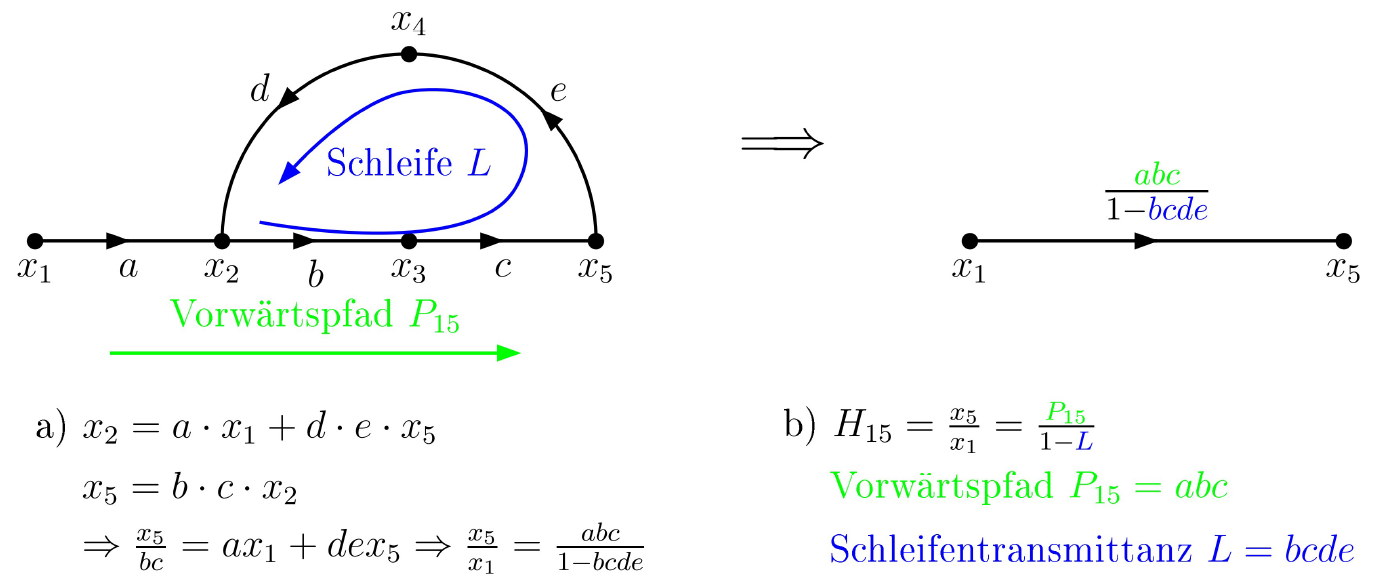
\includegraphics[width=0.9\columnwidth]{images/einzelne_schleife.png}
\end{center}

\columnbreak


\myul{\textbf{Mehrere sich nicht berührende Schleifen}}

\vspace{0.1cm}

Bei einer Kaskade von sich nicht berührenden Schleifen (d.h., dass sie \textbf{keinen gemeinsamen Knoten} haben) ist die gesamte
Transmittanz gegeben durch: 

\vspace{0.2cm}

\begin{minipage}[c]{0.45\columnwidth}
    $$ \boxed{ H_{\rm in} = \frac{P_{ij}}{1-L_j} \cdot\frac{P_{jk}}{1-L_k} \cdot \ldots \cdot \frac{P_{(n-1)n}}{1-L_n} } $$
\end{minipage}
\hfill
\begin{minipage}[c]{0.5\columnwidth}
    \begin{tabular}{ll}
        $H_{\rm in}$& Gesamte Transmittanz              \\ 
        $P_{ij}$    & Transmittanz des Vorwärtspfades   \\
                    & von $x_i$ nach $x_j$              \\
        $L$         & Transmittanz der Schleife 
    \end{tabular}
\end{minipage}

\begin{center}
    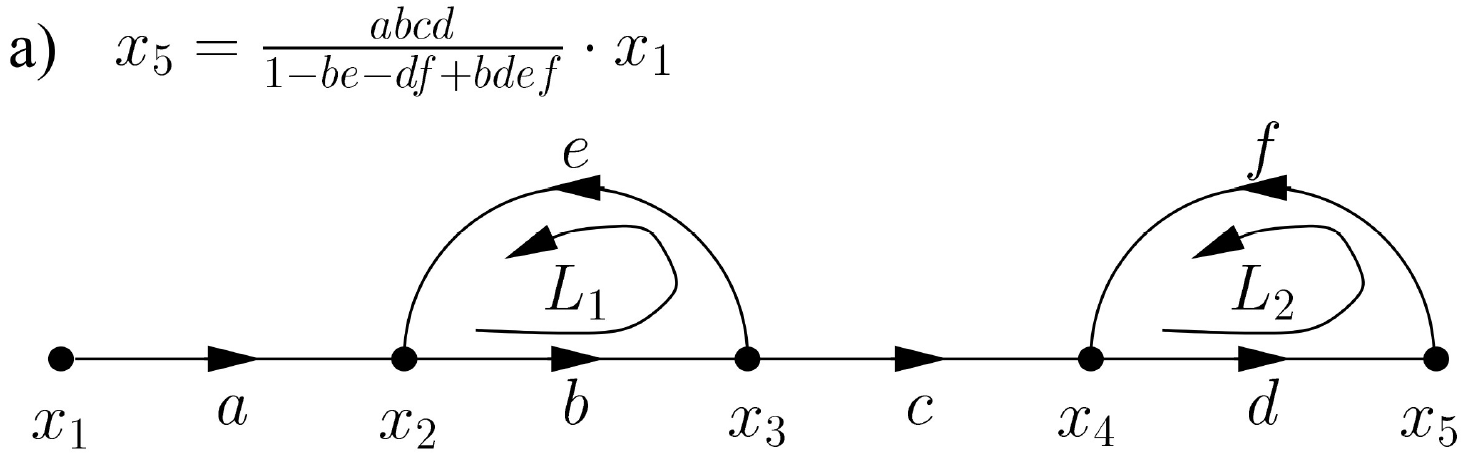
\includegraphics[width=0.8\columnwidth]{images/nicht_beruehrende_schleifen.png}
\end{center}


\myul{\textbf{Mehrere sich berührende Schleifen}}

Für den Fall, dass zwei Schleifen mind. einen \textbf{gemeinsamen Knoten} haben, ist die gesamte Transmittanz gegeben durch:

\begin{center}
    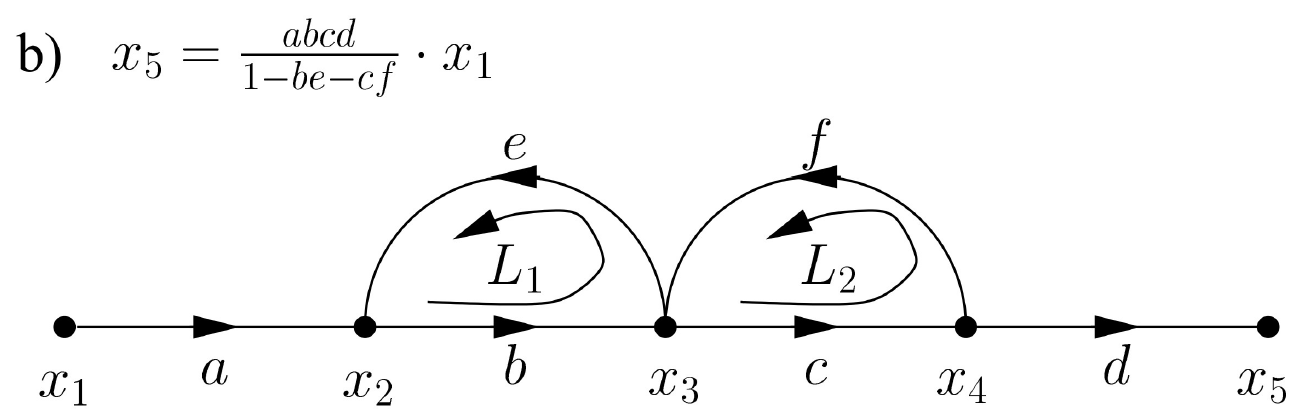
\includegraphics[width=0.8\columnwidth]{images/beruehrende_schleifen.png} 
\end{center}


\subsubsection{Allg. Mehrfachschleifen-Reduktionsregel für einfache Pfade}

Es existiert \textbf{nur ein Pfad} zwischen einer Quelle $x_i$ und einem abhängigen Knoten $x_j$, wobei dieser Pfad jede Schleife
im SFD berührt (d.h., dass er \textbf{wenigstens einen Knoten mit jeder Schleife} gemeinsam hat)

\vspace{0.2cm}

\begin{minipage}{0.25\columnwidth}
    $$ \boxed{ H_{ij} = \frac{x_j}{x_i} = \frac{P_{ij}}{\Delta} } $$
\end{minipage}
\hfill
\begin{minipage}{0.7\columnwidth}
    \begin{tabular}{ll}
        $H_{ij}$    & Gesamte Transmittanz              \\ 
        $P_{ij}$    & Transmittanz des Vorwärtspfades   \\
                    & von $x_i$ nach $x_j$              \\
        $\Delta$    & Graph- / Netzwerkdeterminante
    \end{tabular}
\end{minipage}

\vspace{0.2cm}

\fcolorbox{red}{white}{\parbox{0.97\columnwidth}{
 $\Delta = $ 1 \cor{$-$} (Summe aller Schleifen) \cor{$+$} (Summe aller Produkte zweier Schleifen, die sich \textbf{nicht berühren}) 
    \cor{$-$} (Summe aller Produkte dreier Schleifen, die sich \textbf{nicht berühren}) \cor{$+$} $\ldots$}}
 
\begin{center}
    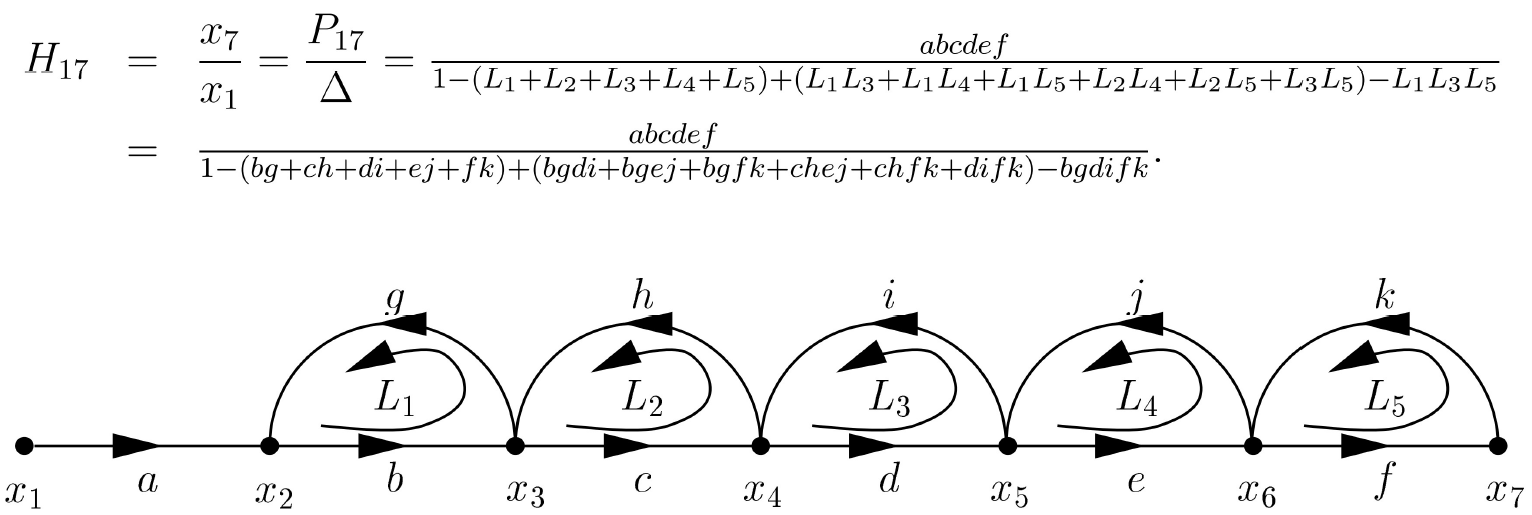
\includegraphics[width=0.9\columnwidth]{images/beispiel_schleifenreduktion.png}
\end{center}

\textrightarrow\ \textbf{Schleifen dürfen auch innerhalb von Schleifen sein}


\subsubsection{Mason's Regel}{27-71}

 
\begin{minipage}{0.4\columnwidth}
    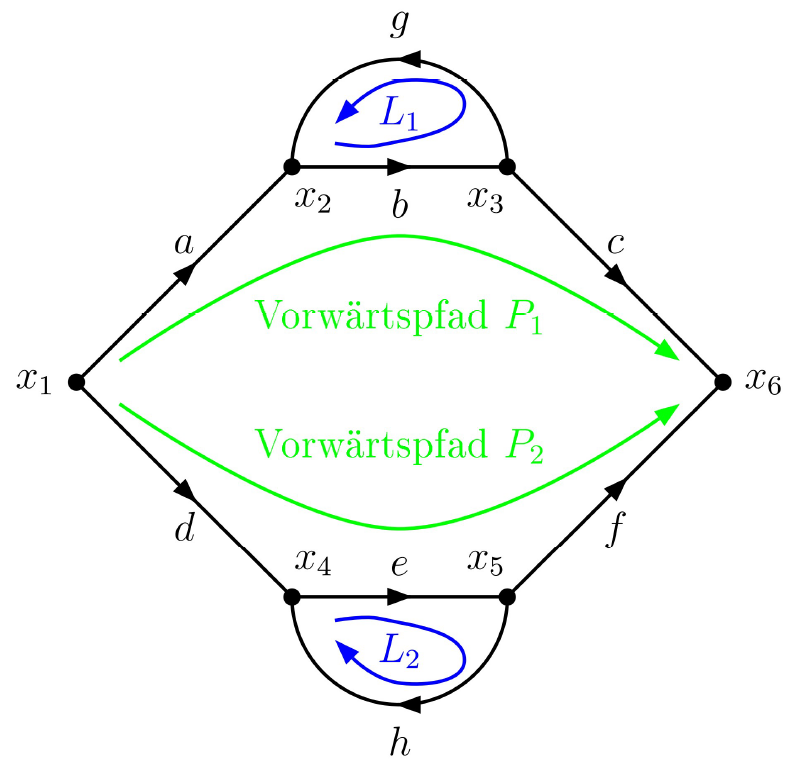
\includegraphics[width=\columnwidth]{images/mason_regel.png}
\end{minipage}
\hfill
\begin{minipage}{0.48\columnwidth}
    \raggedright

    $$ \boxed{ H_{ij} = \frac{x_j}{x_i} = \frac{\sum\limits_k (P_k \cdot \Delta_k )}{\Delta} } $$

    \vspace{0.2cm}

    \crd{\textbf{$x_i$ muss eine Quelle sein!}} \\
    $x_j$ kann eine Senke oder ein gemischter Knoten sein 
\end{minipage}

\vspace{0.2cm}

    \begin{tabular}{ll}
    $H_{ij}$    & Gesamte Transmittanz                                                          \\ 
    $P_{k}$     & Transmittanz des k-ten offenen Pfades zwischen $x_i$ und $x_j$                \\
    $\Delta$    & Graph- / Netzwerkdeterminante                                                 \\
    $\Delta_k$  & Kofaktor (Kodeterminante) \textrightarrow\ siehe \crd{rote} Box               \\
                & Schleifentransmittanzen, welche k-ten Vorwärtspfad \textbf{nicht} berühren    \\
                & \textrightarrow\ siehe \crd{rote} Box
\end{tabular}

\vspace{0.2cm}

\textbf{Es gibt gleich viele Kofaktoren wie Vorwärtspfade}

\vspace{0.2cm}

\textbf{Wenn $\bm{x_i}$ (hier als Beispiel $\bm{x_2}$) keine Quelle ist:} 
$$ \cbl{ H_{23} = \frac{x_3}{x_2} = \frac{\frac{x_3}{x_1}}{\frac{x_2}{x_1}} 
    = \frac{H_{13}}{H_{12}} = \frac{\frac{P_4 \Delta_4 + P_5 \Delta_5}{\Delta}}{\frac{P_1 \Delta_1 + P_2 \Delta_2 + P_3 \Delta_3}{\Delta}} 
    \quad \text{ \textrightarrow\ } \Delta \text{ streicht sich} }$$



\example{Beispiel Mason's Regel}

\begin{center}
    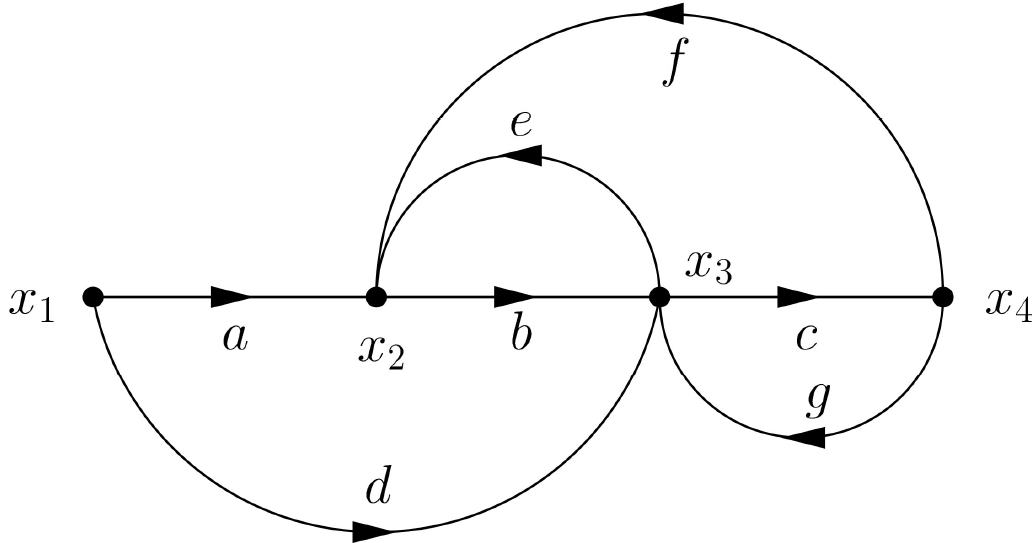
\includegraphics[width=0.65\columnwidth]{images/mason_beispiel_1.png} 
\end{center}


\myul{\textbf{$\bm{x_1}$ ist Quelle:}}

\begin{center}
    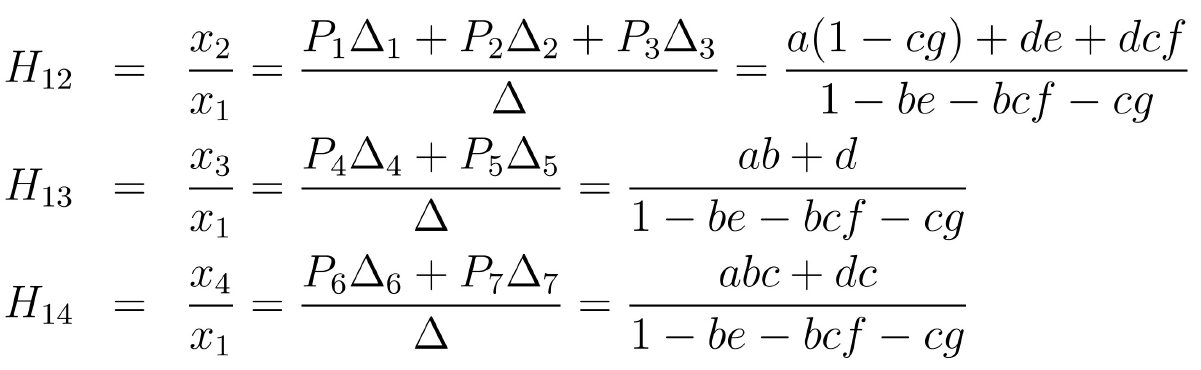
\includegraphics[width=0.8\columnwidth]{images/mason_beispiel_2.png}
\end{center}


\cbl{\myul{\textbf{$\bm{x_2}$ ist keine Quelle:} }}

\vspace{0.2cm}

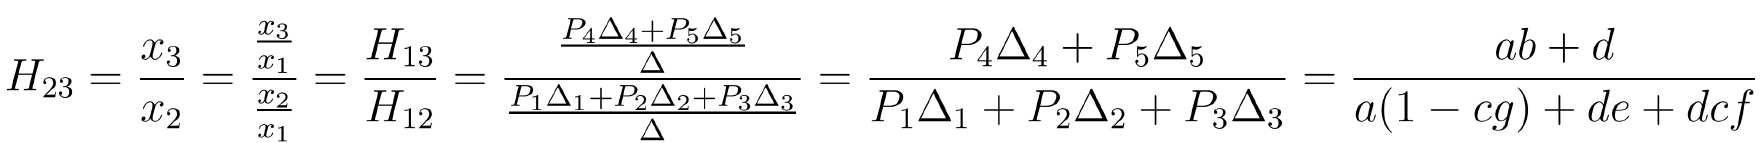
\includegraphics[width=\columnwidth]{images/mason_beispiel_3.png} 


\subsection{Ordnung eines SFD}{72}

Die Ordnung eines SFDs entspricht der \textbf{minimalen Anzahl Knoten}, welche \textbf{entfernt} werden müssen, 
um \textbf{alle Schleifen aufzubrechen}. \\
Diese zu entfernenden Knoten heissen \cbl{\textbf{fundamentale Knoten}} 

\vspace{0.2cm}

\textbf{Hinweis:} 'Entfernen' bedeutet, den Knoten ersatzlos zu streichen (und somit Pfade bzw. die \textbf{Schleifen} zu zerstören)

\begin{center}
    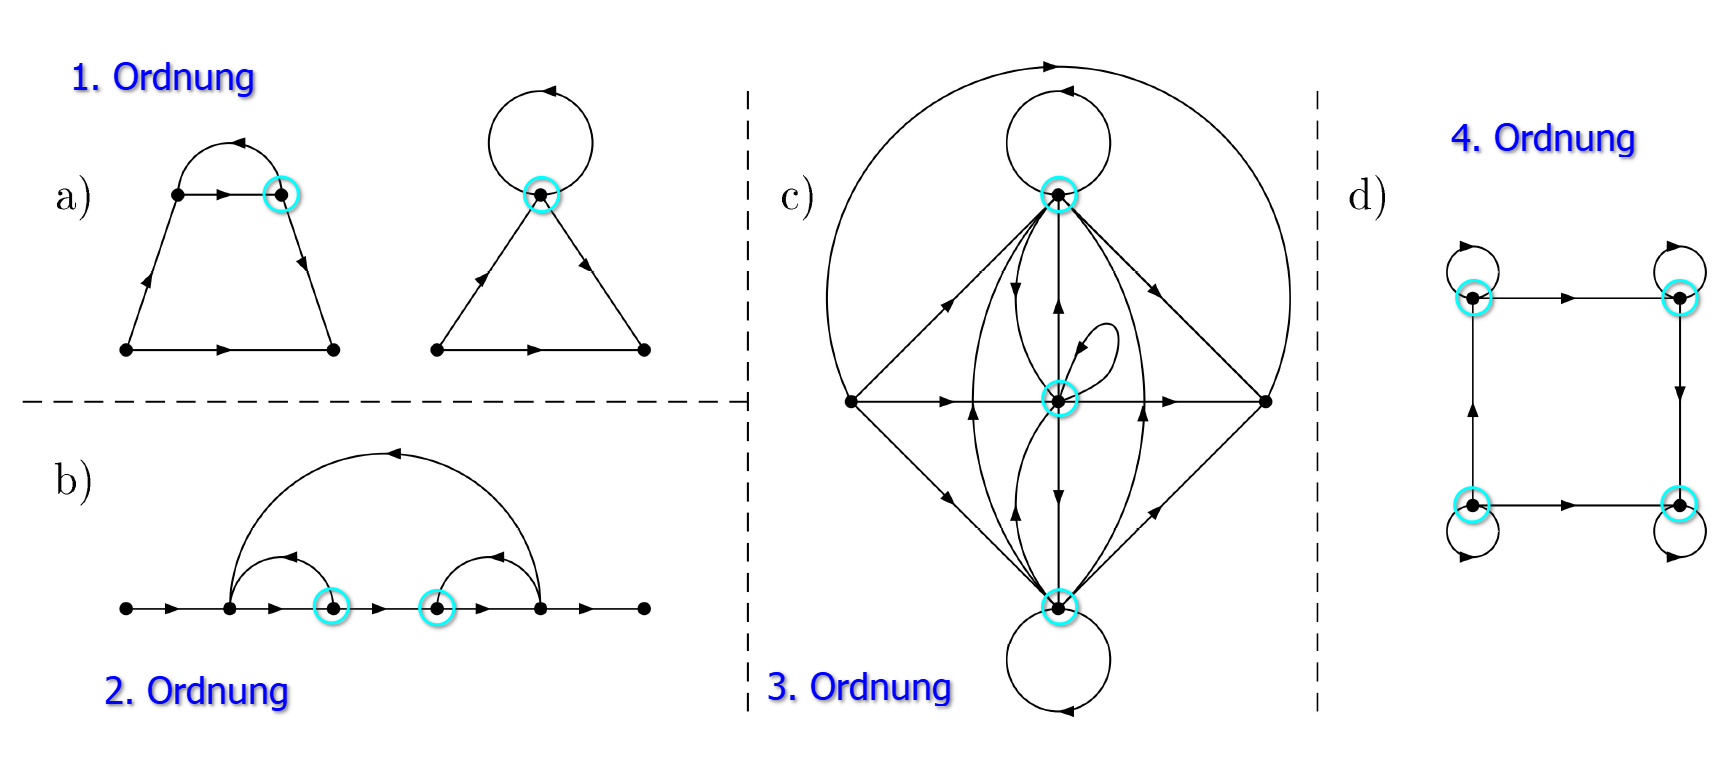
\includegraphics[width=0.9\columnwidth]{images/ordnung_SFD.png}
\end{center}

\textrightarrow\ Die \textbf{Ordnung eines SFDs} entspricht im Allgemeinen \textbf{nicht der Ordnung} des dazugehörigen \textbf{Systems}


\subsection{Fundamentales SFD 1. Ordnung}{73}

\begin{minipage}{0.27\columnwidth}
    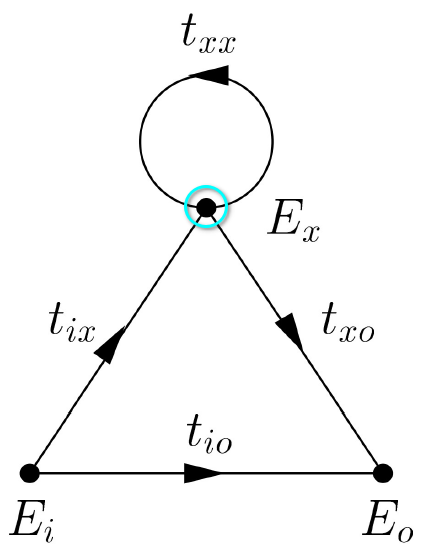
\includegraphics[width=\columnwidth]{images/fundamentales_SFD_ordnung_1.png} 
\end{minipage}
\hfill
\begin{minipage}{0.66\columnwidth}
    \begin{tabular}{ll}
        $E_x$       & Fundamentaler Knoten                      \\
        $E_i$       & Eingangsknoten (Quelle)                   \\
        $E_o$       & Ausgangsknoten (Senke)                    \\
        $t_{io}$    & Totale Transmittanz von $E_i$ zu $E_o$    \\
        $t_{ix}$    & Totale Transmittanz von $E_i$ zu $E_x$    \\
        $t_{xo}$    & Totale Transmittanz von $E_x$ zu $E_o$    \\
        $t_{xx}$    & Totale Transmittanz von $E_x$ zu $E_x$ 
    \end{tabular}
\end{minipage}


\subsubsection{Übertragungsfunktion UTF eines SFD 1. Ordnung}

\vspace{-0.2cm}
$$ \boxed{ H_{io} = \frac{E_o}{E_i} = t_{io} + \frac{t_{ix} \, t_{xo}}{1 - t_{xx}} = 
    \frac{t_{io} - t_{io} \, t_{xx} + t_{ix} \, t_{xo}}{1- t_{xx}}} $$

\textbf{Die Paramteter $\bm{t_{io}}$, $\bm{t_{ix}}$, $\bm{t_{xo}}$ und $\bm{t_{xx}}$ müssen gemäss obiger Tabelle bestimmt werden}


\subsection{Transposition}{85-86}

Die Transposition ist eine wichtige Methode für die Ableitung von \textbf{alternativen praktischen Topologien} mit \textbf{identischen UTF}


\subsubsection{Vorgehen Transposition}

\begin{enumerate}
   \item Richtungsumdrehung aller Zweigtransmittanzen bei gleichbleibenden Transmittanzen 'Pfeile umdrehen' 
   \item Spiegelung des resultierenden SFD
   \item Bezeichnungswechsel von Eingangs- und Ausgangsknoten
\end{enumerate}

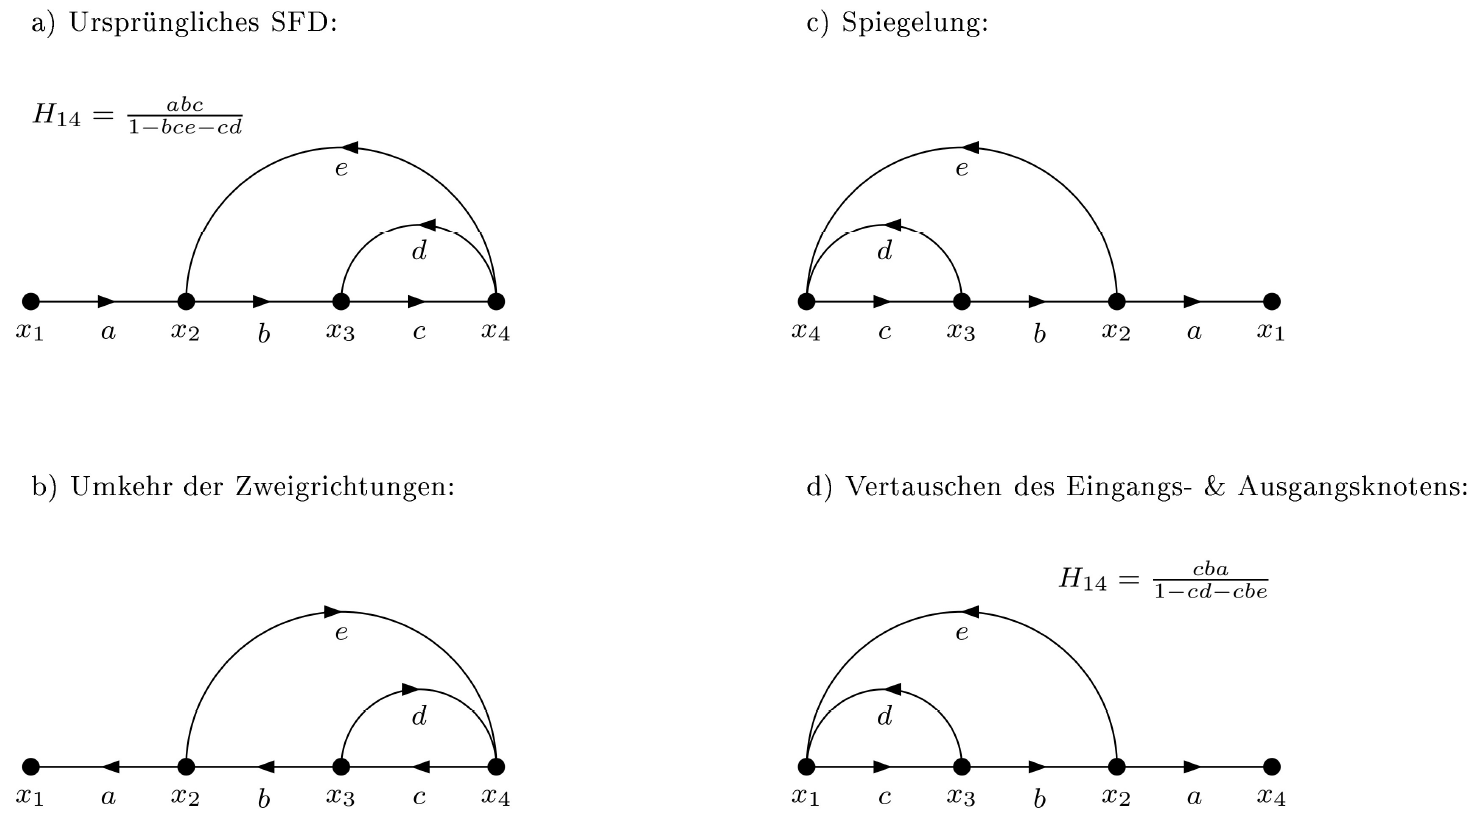
\includegraphics[width=\columnwidth]{images/transposition.png} 


\subsubsection{Inversion vs. Transposition}

Bei der \textbf{Inversion} enthält das resultierende SFD nur noch Vorwärtspfade und keine Rückkopplungsschleifen. \\
Die Resulultierende nichtkausale Funktion ist die Summer aller Pfade von der neuen Quelle zur neuen Senke.

\vspace{0.2cm}

\scalebox{0.9}{
\begin{tabular}{l c c c l}
    $H_{14}$                                                & \textrightarrow\  & Invertierung  & \textrightarrow\  & $\tilde{H}_{41} = \frac{1}{H_{14}}$ \\
    \\
    $ H_{14} = \frac{x_4}{x_1} = \frac{abc}{1-bce - cd} $   &                   &               &                   & $\tilde{H}_{41} = \frac{1}{abc} - \frac{e}{a} - \frac{d}{ba} = \frac{1 - bce - cd}{abc} =  \frac{1}{H_{14}}$ 
    \end{tabular}
}

\vspace{0.2cm}

\begin{center}
    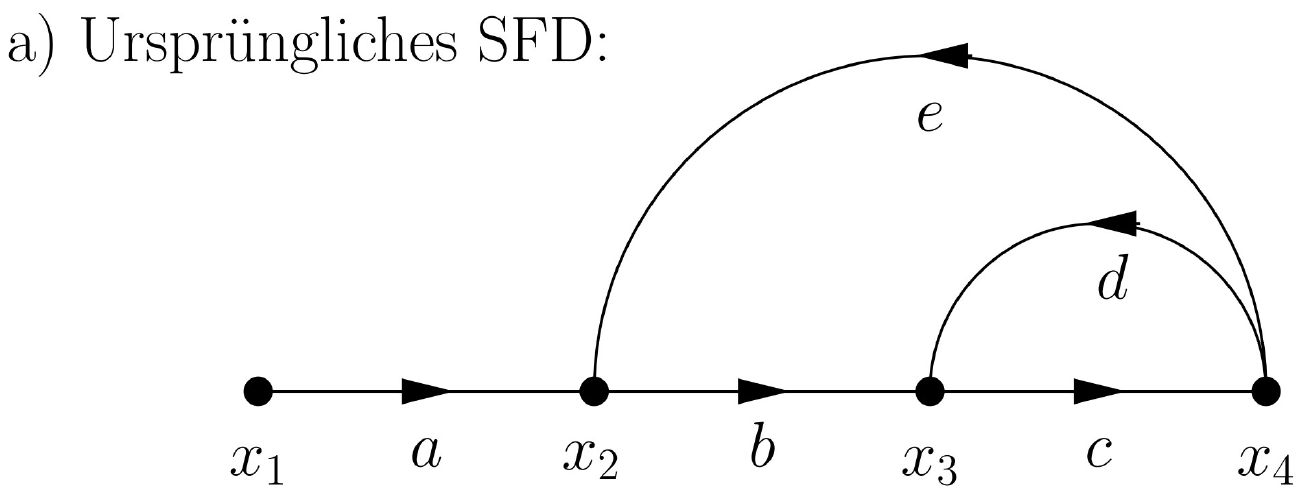
\includegraphics[width=0.45\columnwidth]{images/transposition_vs_invertierung_1.png}
\end{center}

\begin{minipage}[c]{0.48\columnwidth}
    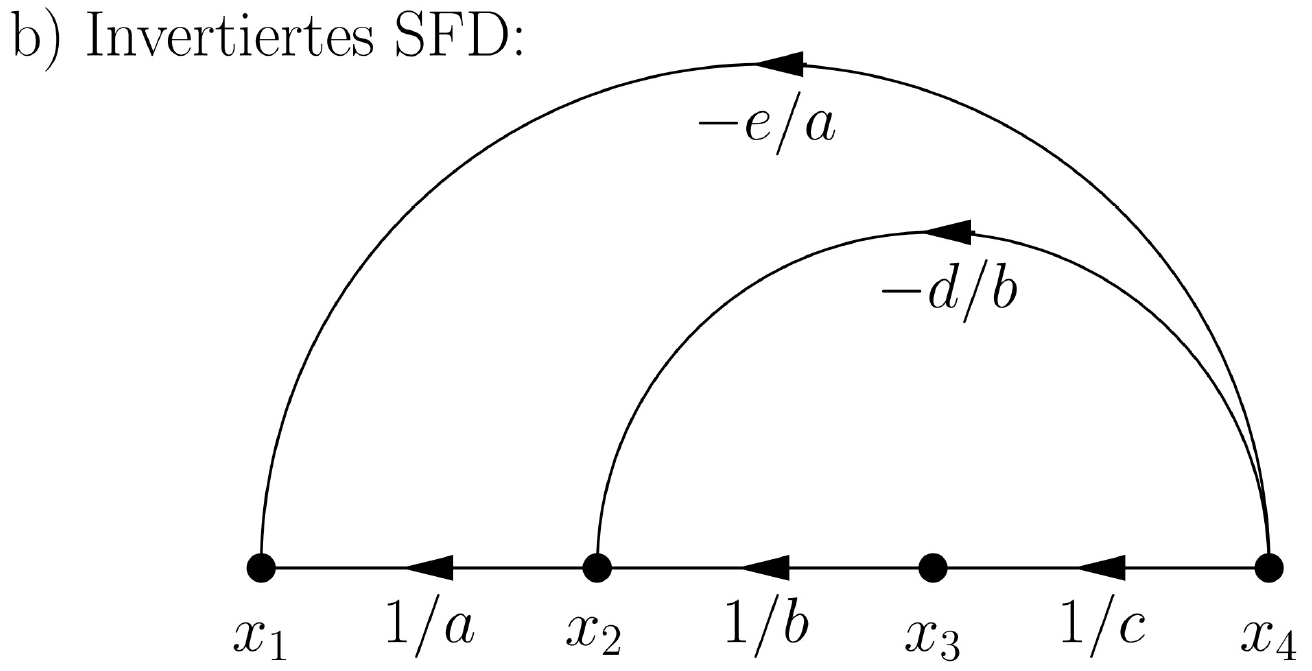
\includegraphics[width=0.9\columnwidth]{images/transposition_vs_invertierung_2.png}
\end{minipage}
\hfill
\begin{minipage}[c]{0.48\columnwidth}
    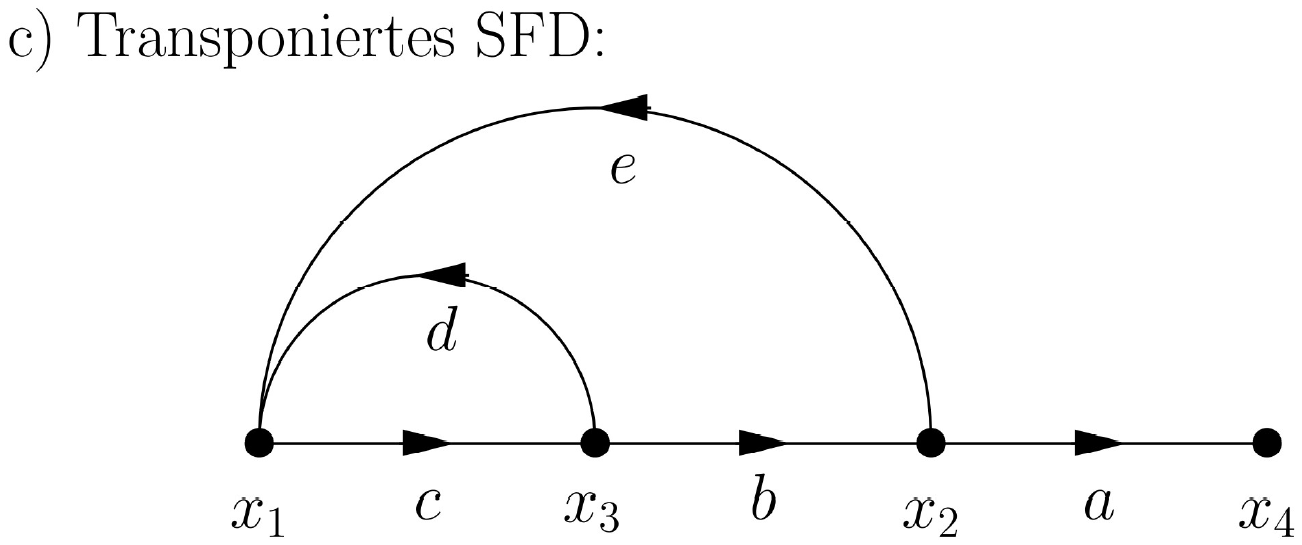
\includegraphics[width=0.95\columnwidth]{images/transposition_vs_invertierung_3.png}
\end{minipage}


\subsection{Skalierung}{86-87}

Ein 'Trennbündel' trennt den Graphen in zwei Mengen $N_a$ und $N_b$ \\
Die Menge $N_a$ enthält dabei den Eingangsknoten 


\subsubsection{Vorgehen Skalierung}

\begin{enumerate}
   \item 'Trennbündel' festlegen
   \item Hineinführende Zweige mit $\lambda$ multiplizieren
   \item Hinausführende Zweige durch $\lambda$ dividieren
   \item Zweige im 'Trennbünde' nicht ändern!
\end{enumerate}

\vspace{0.2cm}

\begin{minipage}{0.5\columnwidth}
    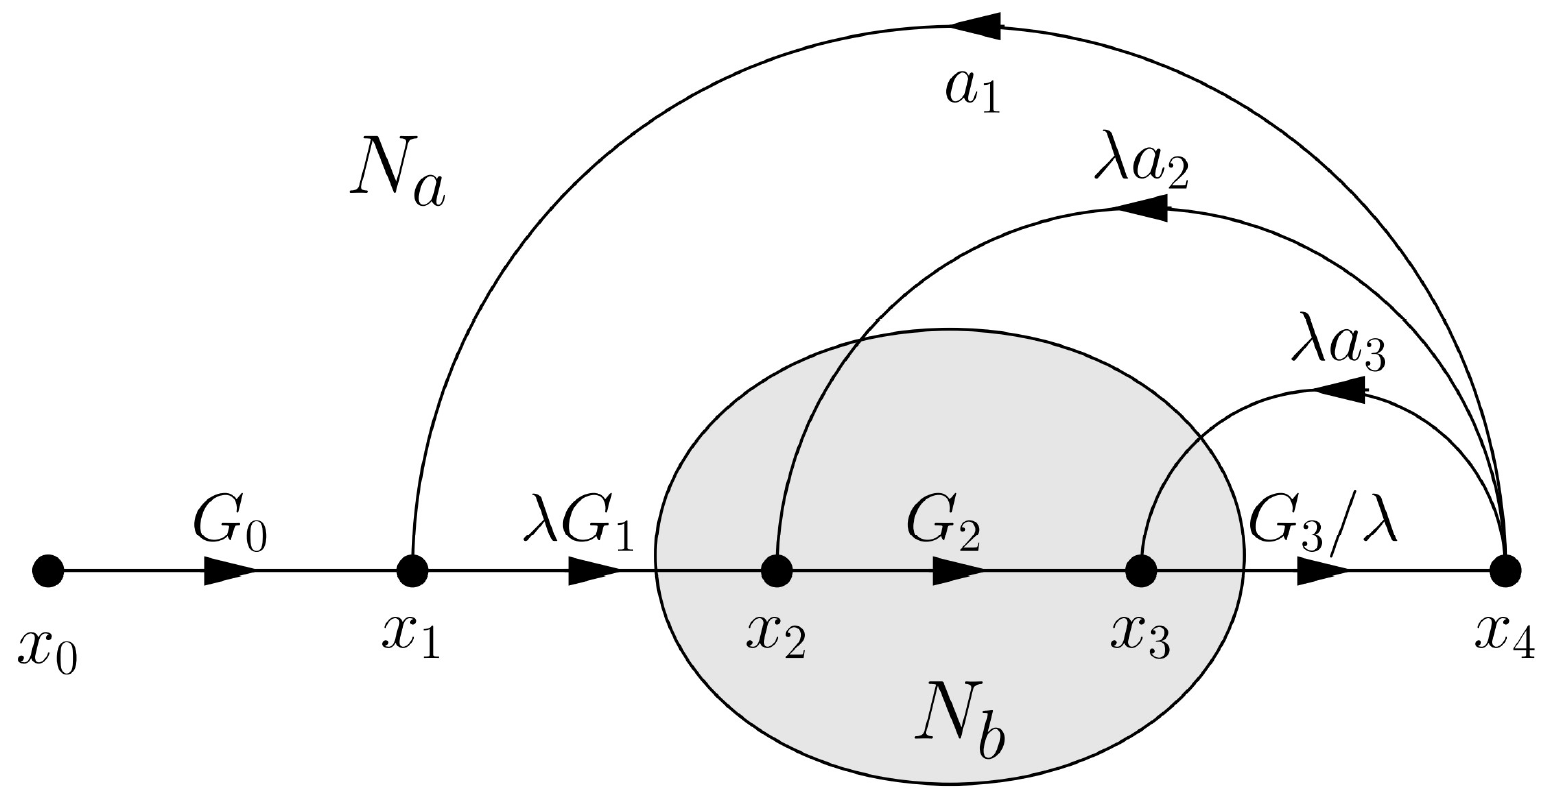
\includegraphics[width=\columnwidth]{images/skalierung.png}
\end{minipage}
\hfill
\begin{minipage}{0.44\columnwidth}
    \raggedright
\textbf{Eine Skalierung ändert die UTF und die Netzwerk-determinante $\bm{\Delta}$ nicht!}
\end{minipage}


\subsection{Anwendung: Operationsverstärker}{78-79}

\begin{center}
    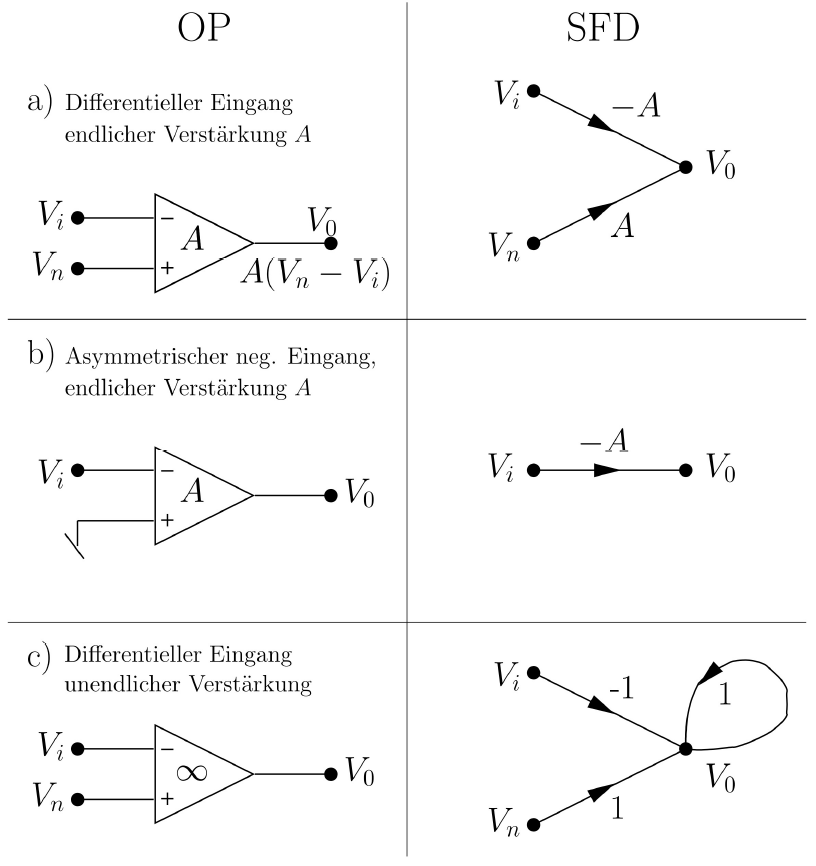
\includegraphics[width=0.7\columnwidth]{images/OPV_als_DFD.png}
\end{center}

